%HW04.tex
%
% Fourth Homework for Graduate Algebra
% Frank Sottile
%%%%%%%%%%%%%%%%%%%%%%%%%%%%%%%%%%%%%%%%%%%%%%%%%%%%%%%%%%%%%%%%%%%%%%%
\documentclass[12pt]{article}
\usepackage{multicol,amsfonts, amssymb,  mathtools,amsmath}
\usepackage{colordvi,graphicx}
\headheight=8pt
%
\topmargin=-75pt
\textheight=720pt   \textwidth=560pt
\oddsidemargin=-60pt \evensidemargin=-60pt
 
\pagestyle{empty}

%%%%%%%%%%%%%%%%%%%%%%%%%%%%%%%%%%%%%%%%%%%%
\newcommand{\CC}{{\mathbb C}}
\newcommand{\KK}{{\mathbb K}}
\newcommand{\NN}{{\mathbb N}}
\newcommand{\QQ}{{\mathbb Q}}
\newcommand{\RR}{{\mathbb R}}
\newcommand{\TT}{{\mathbb T}}
\newcommand{\ZZ}{{\mathbb Z}}

\newcommand{\calA}{{\mathcal A}}

\newcommand{\be}{{\bf e}}
\newcommand{\bfi}{{\bf i}}
\newcommand{\bfj}{{\bf j}}

\newcommand{\Hom}{\mbox{Hom}}
\newcommand{\spec}{\mbox{spec}}
\newcommand{\cone}{\mbox{cone}}

\newcommand{\vect}[2]{(\begin{smallmatrix}#1\\#2\end{smallmatrix})}
\newcommand{\msp}{\hspace{8pt}}
%\newcommand{\Square}{\raisebox{-2pt}{\includegraphics{images/Square.eps}}}
\newcommand{\Square}{\raisebox{-2pt}{\Large$\square$}}

\def\Color#1#2{\special{color push cmyk #1}#2\special{color pop}}
%\def\Indigo#1{\Color{.42 1. 0. .49}{#1}}
\def\Indigo#1{\Color{1. .95 .05 .4}{#1}}
\def\MyViolet#1{\Color{.6 1. 0. .15}{#1}}
\def\TAMU#1{\Color{.15 1. .39 .69}{#1}}

\newcommand{\barsl}{\noindent\begin{minipage}[t]{590pt}
\Indigo{\rule{590pt}{1.2pt}}\vspace{-5.7mm}\\
\MyViolet{\rule{590pt}{1.2pt}}\vspace{-5.7mm}\\
\Blue{\rule{590pt}{1.2pt}}\vspace{-5.7mm}\\
\Green{\rule{590pt}{1.2pt}}\vspace{-5.7mm}\\
\Yellow{\rule{590pt}{1.2pt}}\vspace{-5.7mm}\\
\Orange{\rule{590pt}{1.2pt}}\vspace{-5.7mm}\\
\Red{\rule{590pt}{1.2pt}}\bigskip
\end{minipage}}


\newcommand{\barsn}{\noindent\begin{minipage}[t]{590pt}
\Indigo{\rule{590pt}{1.1pt}}\vspace{-4.5mm}\\
\MyViolet{\rule{590pt}{1.1pt}}\vspace{-4.5mm}\\
\Blue{\rule{590pt}{1.1pt}}\vspace{-4.5mm}\\
\Green{\rule{590pt}{1.1pt}}\vspace{-4.5mm}\\
\Yellow{\rule{590pt}{1.1pt}}\vspace{-4.5mm}\\
\Orange{\rule{590pt}{1.1pt}}\vspace{-4.5mm}\\
\Red{\rule{590pt}{1.1pt}}\bigskip
\end{minipage}}

\def\demph#1{\TAMU{{\sl #1}}}
\def\defcolor#1{\TAMU{#1}}

\begin{document}
\LARGE 
\noindent
Algebra \ \ Autumn 2025\vspace{1pt}\\
Frank Sottile\vspace{2pt}\\
\Large 11 September 2025 \hfill
\sf
 Fourth Homework\makebox[20pt][l]{\ }
\normalsize\vspace{10pt}

\noindent
Write your answers neatly, in complete sentences.  
I highly recommend recopying your work before handing it in.
Correct and crisp proofs are greatly appreciated; oftentimes your work can be shortened and made clearer.

Some problems were partially done in class.
This is an opportunity to polish your skills at writing mathematics in a clear and organized manner.

I am also hoping that this assignment has some easier  problems.
The last homework was a bit more than I probably should assign.

\barsn

\noindent\Maroon{{\sf Hand in at the start of class, Thursday 18 September:}} 



%%%%%%%%%%%%%%%%%%%%%%%%%%%%%%%%%%%%%%%%%%%%%%%%%%%%%%%%%%%%%%%%%%%%%%%%%%%%%%%%%%%%%%%%%%%%%%%%%%%%
\begin{enumerate}
\setcounter{enumi}{20}


%%%%%%%%%%%%%%%%%%%%%%%%%%%%%%%%%%%%%%%%%%%%%%%%%%%%%%%%%%%%%%%%%%%%%%%%%%%%%%%%%%%%%%%%%%%%%%%%%%%%
\item
  Let $G$ be a group with subgroups $H$ and $K$.\vspace{-3pt}
  \begin{enumerate}
   \item Prove that $H\cap K$ is a subgroup of $G$.

   \item If both $H$ and $K$ are normal subgroups of $G$, prove that $H\cap K$ is a normal subgroup of $G$.

   \item If the set $H\cap K$ is replaced by $H\cup K$, do the answers to parts (a) and (b) change?
         Justify your answer.
  \end{enumerate}
%%%%%%%%%%%%%%%%%%%%%%%%%%%%%%%%%%%%%%%%%%%%%%%%%%%%%%%%%%%%%%%%%%%%%%%%%%%%%%%%%%%%%%%%%%%%%%%%%%%%


%%%%%%%%%%%%%%%%%%%%%%%%%%%%%%%%%%%%%%%%%%%%%%%%%%%%%%%%%%%%%%%%%%%%%%%%%%%%%%%%%%%%%%%%%%%%%%%%%%%%
\item Let $G$ be a group.
  Show that its commutator subgroup, $[G,G]$, is a normal subgroup of $G$.

  Show that $G/[G,G]$ is an abelian group.
  This is the \demph{abelianization} of $G$.

  Suppose that $\varphi\colon G \to H$ is a homomorphism of groups with $H$ abelian.
  Show that $[G,G]\subset\ker(\varphi)$.
  Conclude that every homomorphism from $G$ to an abelian group factors through its abelianization.
  
%%%%%%%%%%%%%%%%%%%%%%%%%%%%%%%%%%%%%%%%%%%%%%%%%%%%%%%%%%%%%%%%%%%%%%%%%%%%%%%%%%%%%%%%%%%%%%%%%%%%

%%%%%%%%%%%%%%%%%%%%%%%%%%%%%%%%%%%%%%%%%%%%%%%%%%%%%%%%%%%%%%%%%%%%%%%%%%%%%%%%%%%%%%%%%%%%%%%%%%%%
\item   You will prove  \defcolor{{\bf Gorsat's Lemma}:}
   Let $G_1$ and $G_2$ be groups and suppose that  $H$ is a subgroup of $G_1\times G_2$ whose image under each
    coordinate projection $p_i\colon G_1\times G_2\to G_i$ for $i\in\{1,2\}$ is surjective.
    Let $N_1\subset H$ be the kernel of $p_2$ and $N_2\subset H$ be the kernel of $p_1$ and show that we may identify $N_i$
    as a normal subgroup of $G_i$, for  $i\in\{1,2\}$.

    Finally, show that the image of $H$ in $G_1/N_1 \times G_2/N_2$ is the graph of an isomorphism
    $G_1/N_1 \xrightarrow{\ \sim\ } G_2/N_2$.   
%%%%%%%%%%%%%%%%%%%%%%%%%%%%%%%%%%%%%%%%%%%%%%%%%%%%%%%%%%%%%%%%%%%%%%%%%%%%%%%%%%%%%%%%%%%%%%%%%%%%
 
%%%%%%%%%%%%%%%%%%%%%%%%%%%%%%%%%%%%%%%%%%%%%%%%%%%%%%%%%%%%%%%%%%%%%%%%%%%%%%%%%%%%%%%%%%%%%%%%%%%%
\item  Let $\KK$ be a field.
  Recall that $B(n,\KK)$ is the group of invertible upper triangular matrices with entries in $\KK$.

  Show that $B(2,\KK)$ and $B(3,\KK)$ are solvable.

  (A more elegant route than taken by Lang is to let $U(n,\KK)$ be the subgroup of $B(n,\KK)$ consisting of matrices with
  1s along the diagonal, and explore the commutator subgroup $[U(n,\KK), U(n,\KK)]$.)

%%%%%%%%%%%%%%%%%%%%%%%%%%%%%%%%%%%%%%%%%%%%%%%%%%%%%%%%%%%%%%%%%%%%%%%%%%%%%%%%%%%%%%%%%%%%%%%%%%%%
 
%%%%%%%%%%%%%%%%%%%%%%%%%%%%%%%%%%%%%%%%%%%%%%%%%%%%%%%%%%%%%%%%%%%%%%%%%%%%%%%%%%%%%%%%%%%%%%%%%%%%
\item 
  Give two different composition series for the quaternion group $Q_8$ and verify that they are equivalent
  (\`a la Jordan-H\"older).
  Also, verify that $Q_8$ is solvable.
%%%%%%%%%%%%%%%%%%%%%%%%%%%%%%%%%%%%%%%%%%%%%%%%%%%%%%%%%%%%%%%%%%%%%%%%%%%%%%%%%%%%%%%%%%%%%%%%%%%%
    

%%%%%%%%%%%%%%%%%%%%%%%%%%%%%%%%%%%%%%%%%%%%%%%%%%%%%%%%%%%%%%%%%%%%%%%%%%%%%%%%%%%%%%%%%%%%%%%%%%%%
\item
  Repeat the previous question, but for the dihedral group of order 8.
%%%%%%%%%%%%%%%%%%%%%%%%%%%%%%%%%%%%%%%%%%%%%%%%%%%%%%%%%%%%%%%%%%%%%%%%%%%%%%%%%%%%%%%%%%%%%%%%%%%%

%%%%%%%%%%%%%%%%%%%%%%%%%%%%%%%%%%%%%%%%%%%%%%%%%%%%%%%%%%%%%%%%%%%%%%%%%%%%%%%%%%%%%%%%%%%%%%%%%%%%
\item Please give a complete proof of Theorem 3.2 in Lang:

  Let $G$ be a group with normal subgroup $H$.
  Then $G$ is solvable if and only if both $H$ and $G/H$ are solvable.
%%%%%%%%%%%%%%%%%%%%%%%%%%%%%%%%%%%%%%%%%%%%%%%%%%%%%%%%%%%%%%%%%%%%%%%%%%%%%%%%%%%%%%%%%%%%%%%%%%%%


      
\end{enumerate}
%%%%%%%%%%%%%%%%%%%%%%%%%%%%%%%%%%%%%%%%%%%%%%%%%%%%%%%%%%%%%%%%%%%%%%%%%%%%%%%%%%%%%%%%%%%%%%%%%%%%

\end{document}

%%%%%%%%%%%%%%%%%%%%%%%%%%%%%%%%%%%%%%%%%%%%%%%%%%%%%%%%%%%%%%%%%%%%%%%%%%%%%%%%%%%%%%%%%%%%%%%%%%%%
 \item 
%%%%%%%%%%%%%%%%%%%%%%%%%%%%%%%%%%%%%%%%%%%%%%%%%%%%%%%%%%%%%%%%%%%%%%%%%%%%%%%%%%%%%%%%%%%%%%%%%%%%
